\label{fs-acker-preliminaries}

First, in this section, we formalize the properties that should provide a substream management technique. After that, we outline the punctuations framework that is commonly applied in state-of-the-art SPEs. In the last part of this section, we discuss the limitations of the punctuations framework and demonstrate the theoretical lower bound on the overhead induced by a substream management technique.

\subsection{Processing model}

Typically, distributed stream processing engines are shared-nothing runtimes that continuously ingest input elements, transform them according to a logical dataflow graph, and deliver output elements. The logical dataflow graph consists of user-defined operators. Operators can be stateless or stateful: an output element may depend on the current state and the corresponding input element. A logical graph is mapped to a physical, distributed graph upon deployment. Commonly, a single logical operator can be deployed on multiple computational nodes. Further, we denote physical instances of logical operators as {\em processes}.

Distributes SPEs can be modeled~\cite{carbone2018scalable} as physical dataflow graph $G=\{\Pi,\mathcal{E}\}$, where $\Pi$ are processes (deployed operators) and $\mathcal{E} \subseteq \Pi \times \Pi$ are FIFO network channels between them, $c_{ij}=(q,p)\in \mathcal{E}; q,p \in \Pi$. Each process has input channels $I_p = \bigcup_{q \in \Pi} \{c_{qp} | (q,p) \in \mathcal{E}\}$.

Network channels state (all in-transit messages) is denoted as $M$. Each process $p$ can handle elements $m\in M$ from its input channels, e.g. an input element $m_{qp}$ arrives from a process $q$ at a process $p$. On element receiving, process puts it to a {\em sendbox} $B_p$. We denote this event as $\langle recv,m_{qp}\rangle$:

$$\langle recv,m_{qp}\rangle, q\in I_p, M:=M\setminus{m_{qp}}, B_p:=B_p\cup\{m_{qp}\}$$

The transition between sendbox and processing is managed by a {\em sendbox procedure} $S(B)$. Each input event triggers procedure $S(B)$ that can generate the following events in turn:

\begin{enumerate}
    \item Processing: $\langle proc,m_{qp}\rangle, m_{qp}\in B_p$
    \item Substream termination: $\langle eoss,pred(m)\rangle$
\end{enumerate}

Predicate $pred(m)$ defines a substream: it is true if an element $m$ belongs to the substream~\cite{Tucker:2003:EPS:776752.776780}. Each element can belong to multiple substreams at the same time if it satisfies all corresponding predicates. 

A handler of these events is defined by a user or an SPE itself. It can be a user-defined operator, e.g., join, or internal SPE functionality, e.g., state snapshotting procedure. We omit the explicit definition of output elements to simplify the model. Note that all events within the same process $p$ are totally ordered by a local causal order relation $<_p$: $e^{0}_p,e^{1}_p,...,e^{i}_p,...$.

\subsection{Lifespan events}

\subsubsection{Soft bound}

Many applications that apply substream management systems do not require any special properties of termination events. In this case, we denote the guarantee provided by such events as {\em soft bound}, because termination events indicate only the fact that the substream ended some time ago, and other input elements could be processed after that. More formally, we define the soft bound guarantee of the termination event (end-of-substream) $\langle eoss_{soft}, pred(m)\rangle$ as follows:

\begin{align*}
\forall e^{'} = \langle proc,m\rangle, e^{'} >_p \langle eoss_{soft}, pred(m)\rangle : \neg pred(m)
\end{align*}

Figure~\ref{general_guarantees} illustrates this notion. Terms $a,b,c,d...$ denote ordered processing events of a process $p$. The substream ends after event $c$. Note that there are several other events between the end-of-substream and $c$. This is the property of a {\em soft bound} guarantee: if $\langle eoss, pred(m)\rangle$ occurs, all subsequent elements do not satisfy the predicate, but it is not necessarily the exact substream ``border''.

\begin{figure}[htbp]
  \centering
  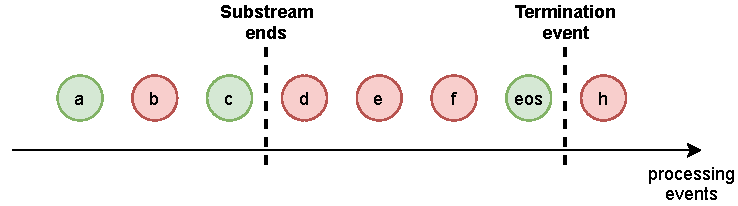
\includegraphics[width=0.50\textwidth]{pics/general-guarantee.pdf}
  \caption{Substream management: soft bound}
  \label{general_guarantees}
\end{figure}

\subsubsection{Firm bound}

The guarantee that any new event will not satisfy the predicate is sufficient for many real-life problems, e.g., SPE can initiate process state pruning on such events. However, some problems require a {\em firm bound}: guarantee that the substream ends {\em exactly} after the termination event. 

For example, epoch-based snapshotting protocol~\cite{2015arXiv150608603C, jacques2016consistent} bases on a notion of {\em epoch}. Epoch is a special substream that should be atomically processed. Therefore, SPE requires the termination event for an epoch that occurs right after the last processing event for this epoch. Otherwise, the snapshot can be inconsistent, because it captures elements from various epochs. To support such scenarios, the end-of-substream event $\langle eoss_{firm}, pred(m)\rangle$ should satsify the following conditions:

\begin{align*}
&1. \forall e^{'} = \langle proc,m\rangle, e^{'} >_p \langle eoss_{firm}, pred(m)\rangle : \neg pred(m) \\
&\boldsymbol{2. \forall e^{*} = \langle proc,m\rangle, e^{*} <_p \langle eoss_{firm}, pred(m)\rangle : pred(m)} \\
\end{align*}

The first condition is the same as for the soft bound guarantee. The second one allows a process to determine the exact processing event when the substream terminates: all elements after the termination event will not satisfy the predicate, but all previous elements have been satisfied. 

Figure~\ref{strict_guarantees} illustrates the notion of the firm bound. As in the previous example, terms $a,b,c,d...$ denote ordered processing events of a process $p$. However, in this case, event $\langle eoss_{firm}, pred(m)\rangle$ occurs right after the substream terminates.

\begin{figure}[htbp]
  \centering
  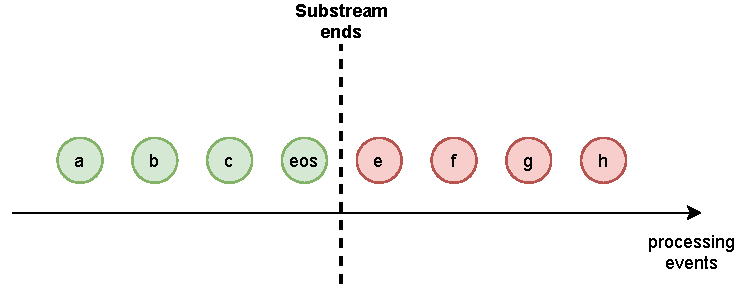
\includegraphics[width=0.50\textwidth]{pics/strict-guarantee.pdf}
  \caption{Substream management: firm bound}
  \label{strict_guarantees}
\end{figure}

\subsubsection{Consistent termination events order}
Some specific applications, including the mentioned earlier epoch-based snapshotting method and techniques for enforcing deterministic processing~\cite{we2018adbis} require an order of termination events to be synchronized with the order of substreams endings (events from data sources). For example, if termination events are reordered, then snapshots for consecutive epochs can be inconsistent. Another example is deterministic join that also requires the defined order of termination events~\cite{gulisano2016scalejoin}.

\begin{figure}[htbp]
  \centering
  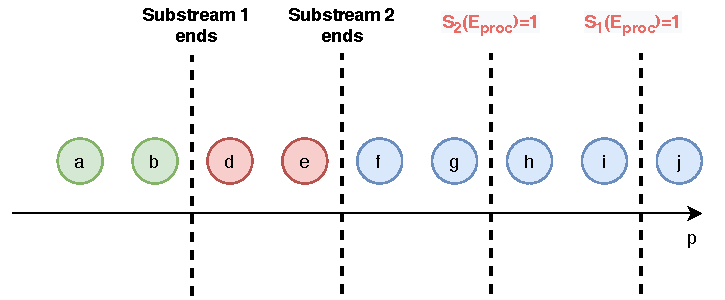
\includegraphics[width=0.50\textwidth]{pics/notifications-reordering.pdf}
  \caption{An example of termination events reordering}
  \label{notifications_reordering}
\end{figure}

Termination events reordering in case of the soft bound guarantee is illustrated in Figure~\ref{notifications_reordering}. Terms $a,b,c,d...$ denote ordered processing events of a process $p$. Although the substream containing events $a,b$ terminates earlier, the end-of-substream event for this substream occurs after the termination event for the substream containing events $d,e$. 

Let $e^{*}_1$ and $e^{*}_2$ be the last elements of substreams defined by predicates $pred_1(m)$ and $pred_2(m)$. Termination events $\langle eoss, pred_1(m)\rangle$ and $\langle eoss, pred_2(m)\rangle$ are {\em consistently ordered} iff:

\begin{align*}
e^{*}_1 >_p e^{*}_2 \Longrightarrow \langle eoss, pred_1(m)\rangle >_p \langle eoss, pred_2(m)\rangle
\end{align*}

\subsection{Punctuations framework}

\subsubsection{Framework overview}

The main idea behind the punctuations framework is to divide the stream into substreams by injection of special elements that bear predicate $punct$. Punctuations are injected directly into a system as ordinary data elements by SPE or by external data producers. The injector promises that all further produced records do not satisfy the predicate. Hence, the punctuation itself defines the ``border'' of a substream.

Figure~\ref{punctuations_scheme} illustrates the punctuations framework. Green elements indicate elements that belong to some substream, while red elements do not. As we can see, punctuations play the role of delimiter between the substream elements and all further items.

\begin{figure}[htbp]
  \centering
  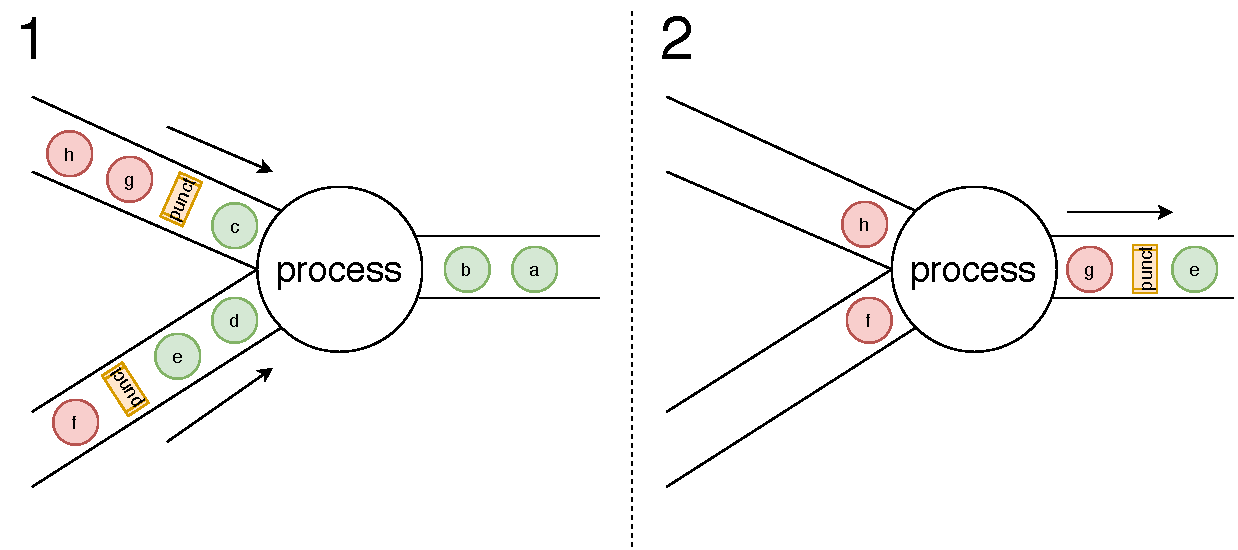
\includegraphics[width=0.50\textwidth]{pics/punctuations-scheme.pdf}
  \caption{Punctuations framework: an example}
  \label{punctuations_scheme}
\end{figure}

Processes within SPE do not apply user-defined operators to punctuations. Instead, each process propagates punctuation to all outgoing channels when it receives corresponding punctuations from all input channels. If a process receives punctuations from all inputs, it is guaranteed that it will not receive elements that satisfy the predicate further due to FIFO network channels. Hence, the formal condition of soft bound termination event $\langle eoss_{soft}, pred(m)\rangle$ is the following:

\begin{align*}
& \langle eoss_{soft}, pred(m)\rangle \Longleftrightarrow \\ 
& \forall q \in I_p, \exists punct_{qp} \in B_p, \forall m\in B : \neg pred(m)
\end{align*}

To satisfy the firm bound guarantee, one needs to hold elements in the sendbox until all punctuations have arrived from all input channels. In~\cite{Carbone:2017:SMA:3137765.3137777} such behavior is called {\em watermark (punctuation) alignment}. More formally, the sendbox procedure should ensure the following order of elements processing to achieve firm bound:

\begin{align*}
& \exists q \in I_p, e = \langle recv,m_{qp} \rangle >_p e^{'} = \langle recv,punct_{qp}\rangle \Longrightarrow \\ 
& <proc, m_{qp}> >_p \langle eoss_{soft}, pred(m)\rangle
\end{align*}

If this condition is satisfied, then $\langle eoss_{firm}, pred(m)\rangle$ = $\langle eoss_{soft}, pred(m)\rangle$ for the punctuations. The punctuations framework provides consistent termination events order by design because punctuations are naturally ordered with ordinary data elements within the processes.

\subsection{Discussion}

\subsubsection{Limitations of punctuations}

While the punctuations approach is robust and easy-to-implement, it has several limitations. In the punctuations framework, the information about the ending of a substream is propagated using ordinary data elements via the data flow network channels. It implies that punctuations are not applicable for cyclic dataflows because a process that receives elements from a cyclic channel will never receive punctuations from this channel~\cite{carbone2018scalable}.

The high network overhead forms another limitation. This method's amount of service traffic is $O(K||\Pi||^2)$, where $||\Pi||$ is the number of processes and $K$ is the number of substreams. As we can see, this estimation is far from the lower bound ($O(||\Pi||)$). It is quadratic in the number of processes, as each process should propagate punctuations to all output channels. 

Substreams can be {\em fine-grained}: for example, each processing key can spawn a substream within a state pruning problem. If there are a lot of small substreams, an inefficient substream management system can reduce the throughput of an SPE itself~\cite{Li:2008:OPN:1453856.1453890} or affect the performance of state checkpointing~\cite{zhang2021research}. As we demonstrate further, the punctuation technique adds significant performance overhead on regular processing for small substreams (frequent punctuations injection).

\subsubsection{Optimal traffic overhead}

A vital performance property of a substream management system is the amount of extra network traffic. Let $||\Pi||$ be a number of processes, and $K$ be a number of substreams. 

\begin{lemma}
The network overhead induced by a substream management system cannot be lower than $O(K||\Pi||)$. 
\end{lemma}
\begin{proof}
When a substream management system detects the end of a substream, it should inform processes about that. In a general case, e.g., for a state snapshotting problem, it should inform all (stateful) processes. Hence, at least one network message (termination notification) must be sent to each process for each substream.
\end{proof}

Despite this lemma's simplicity, we will further use it to figure out how far is some substream management system from this bound. We can also claim a solution as {\em optimal} if its extra traffic estimation is equal to the lower bound from the lemma. In the next sections, we demonstrate that it is possible to design a substream management system that achieves optimal network traffic overhead.
